\documentclass{standalone}
\usepackage{tikz}
\usetikzlibrary{patterns, positioning}
\usepackage[sfdefault]{ClearSans} %% option 'sfdefault' activates Clear Sans as the default text font
\usepackage[T1]{fontenc}

\begin{document}
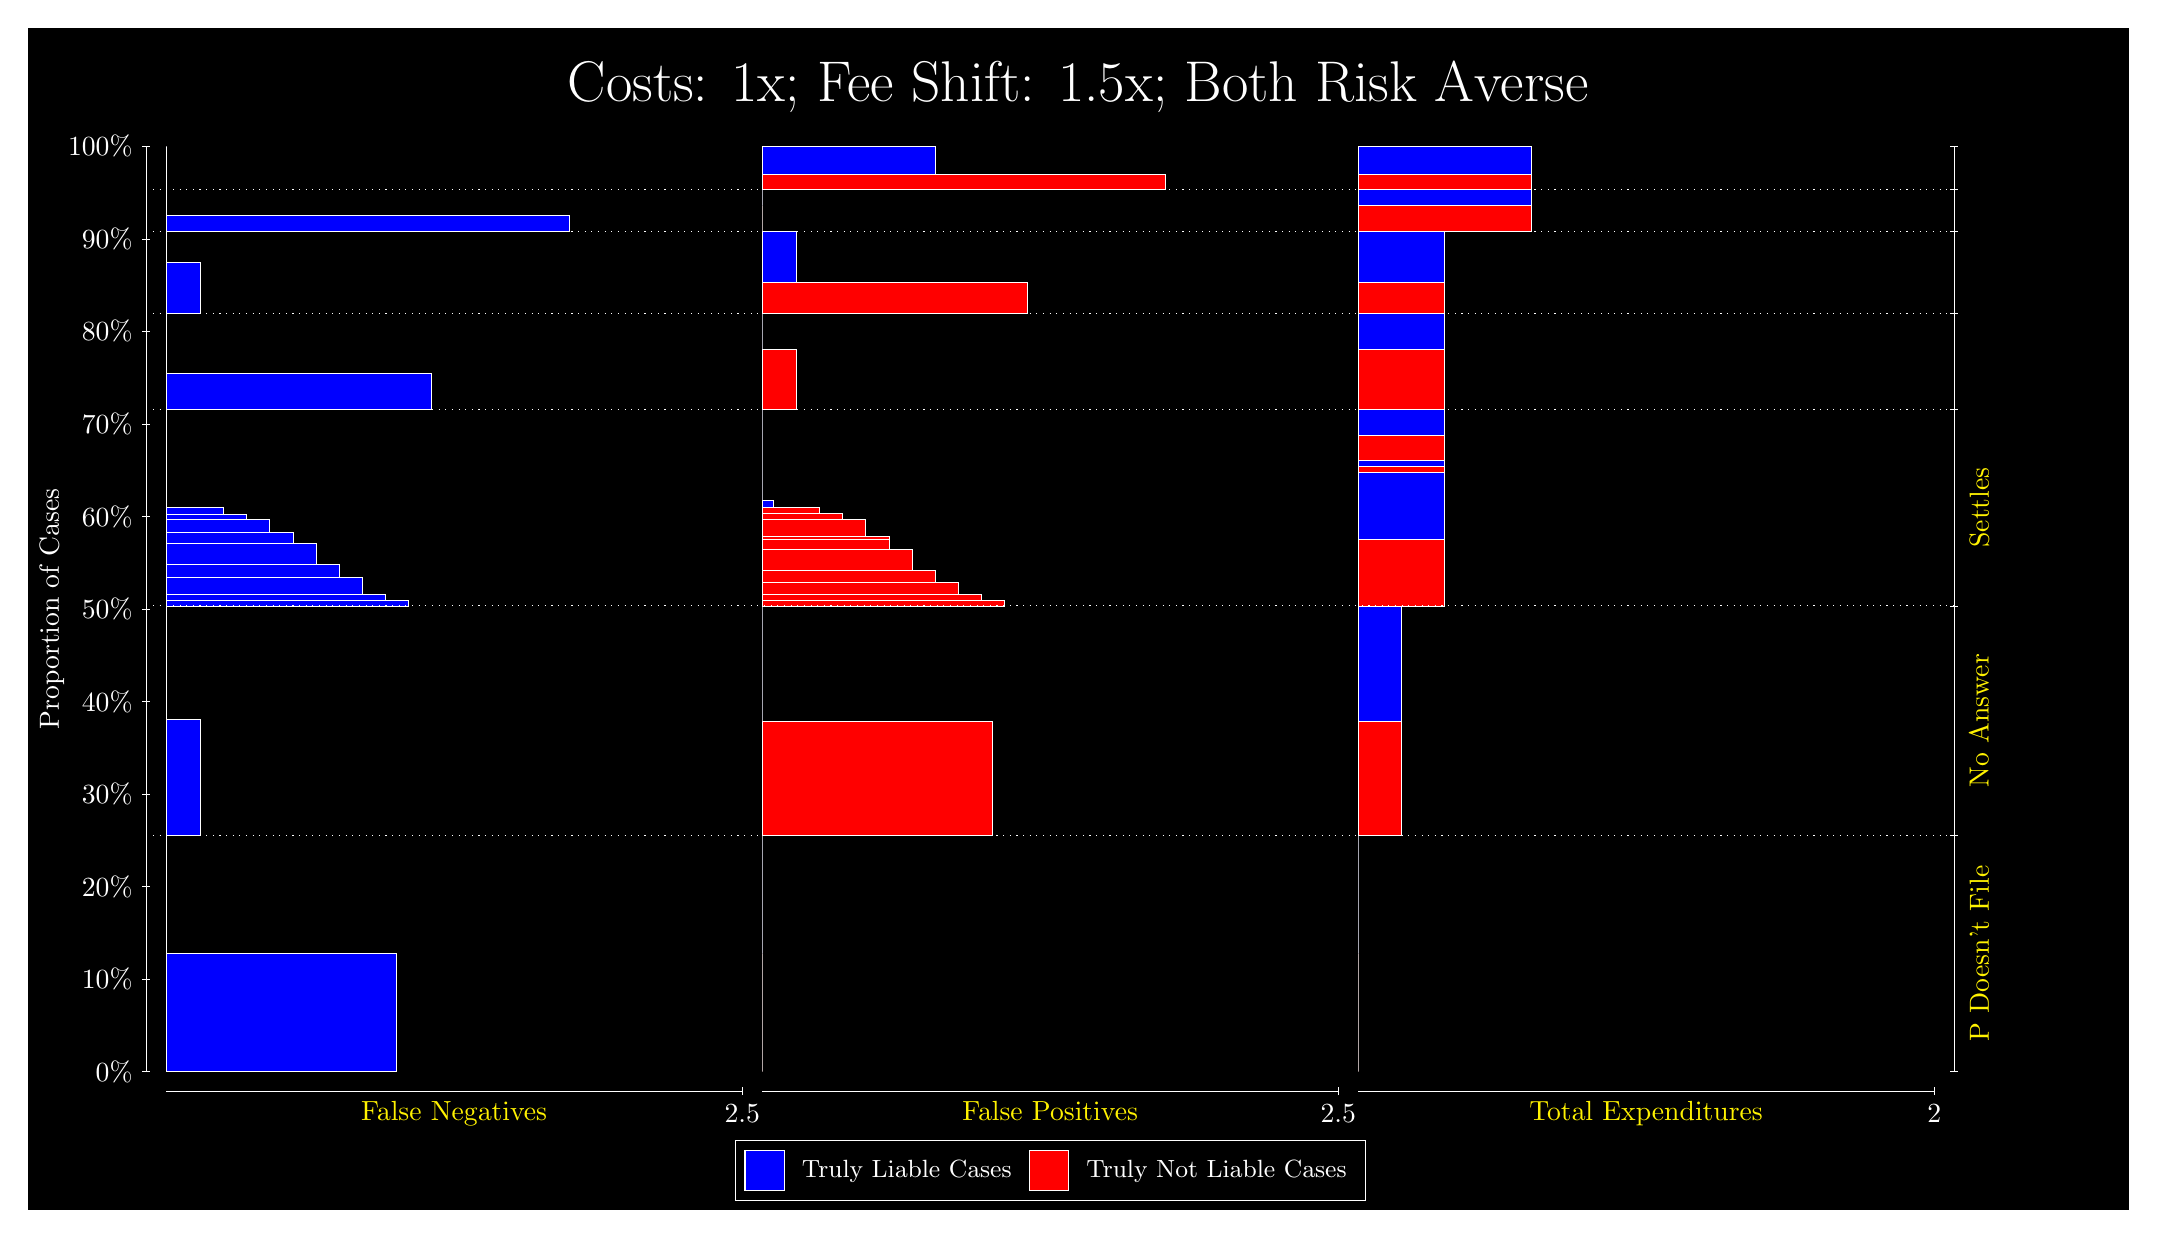
\begin{tikzpicture}
\draw[fill=black] (0,0) rectangle (26.667,15);
\draw[text=white] (0,13.5) rectangle (26.667,15) node[midway] {\huge Costs: 1x; Fee Shift: 1.5x; Both Risk Averse};
\draw[white, very thin] (1.5,1.75) -- (1.5,13.5);
\node[rotate=90, text=white, anchor=center] at (0.3, 7.625) {Proportion of Cases};
\draw[white, very thin] (1.45,1.75) -- (1.55,1.75);
\node[text=white, anchor=east] at (1.45, 1.75) {0\%};
\draw[white, very thin] (1.45,2.925) -- (1.55,2.925);
\node[text=white, anchor=east] at (1.45, 2.925) {10\%};
\draw[white, very thin] (1.45,4.1) -- (1.55,4.1);
\node[text=white, anchor=east] at (1.45, 4.1) {20\%};
\draw[white, very thin] (1.45,5.275) -- (1.55,5.275);
\node[text=white, anchor=east] at (1.45, 5.275) {30\%};
\draw[white, very thin] (1.45,6.45) -- (1.55,6.45);
\node[text=white, anchor=east] at (1.45, 6.45) {40\%};
\draw[white, very thin] (1.45,7.625) -- (1.55,7.625);
\node[text=white, anchor=east] at (1.45, 7.625) {50\%};
\draw[white, very thin] (1.45,8.8) -- (1.55,8.8);
\node[text=white, anchor=east] at (1.45, 8.8) {60\%};
\draw[white, very thin] (1.45,9.975) -- (1.55,9.975);
\node[text=white, anchor=east] at (1.45, 9.975) {70\%};
\draw[white, very thin] (1.45,11.15) -- (1.55,11.15);
\node[text=white, anchor=east] at (1.45, 11.15) {80\%};
\draw[white, very thin] (1.45,12.325) -- (1.55,12.325);
\node[text=white, anchor=east] at (1.45, 12.325) {90\%};
\draw[white, very thin] (1.45,13.5) -- (1.55,13.5);
\node[text=white, anchor=east] at (1.45, 13.5) {100\%};

\draw[white, very thin] (24.457,1.75) -- (24.457,13.5);
\draw[white, very thin] (24.407,1.75) -- (24.507,1.75);
\node[anchor=west] at (24.407, 1.75) {};
\draw[white, very thin] (24.407,4.751) -- (24.507,4.751);
\node[anchor=west] at (24.407, 4.751) {};
\draw[white, very thin] (24.407,7.665) -- (24.507,7.665);
\node[anchor=west] at (24.407, 7.665) {};
\draw[white, very thin] (24.407,10.162) -- (24.507,10.162);
\node[anchor=west] at (24.407, 10.162) {};
\draw[white, very thin] (24.407,11.38) -- (24.507,11.38);
\node[anchor=west] at (24.407, 11.38) {};
\draw[white, very thin] (24.407,12.416) -- (24.507,12.416);
\node[anchor=west] at (24.407, 12.416) {};
\draw[white, very thin] (24.407,12.952) -- (24.507,12.952);
\node[anchor=west] at (24.407, 12.952) {};
\draw[white, very thin] (24.407,13.5) -- (24.507,13.5);
\node[anchor=west] at (24.407, 13.5) {};

\draw[white, very thin, fill=blue] (1.75,1.75) rectangle (4.6775,3.2505);
\draw[white, very thin, fill=red] (1.75,3.2505) rectangle (1.75,4.751);
\draw[white, very thin, fill=blue] (1.75,4.751) rectangle (2.1891,6.2229);
\draw[white, very thin, fill=red] (1.75,6.2229) rectangle (1.75,7.665);
\draw[white, very thin, fill=blue] (1.75,7.665) rectangle (4.8239,7.7304);
\draw[white, very thin, fill=blue] (1.75,7.7304) rectangle (4.5312,7.8079);
\draw[white, very thin, fill=blue] (1.75,7.8079) rectangle (4.2384,8.0254);
\draw[white, very thin, fill=blue] (1.75,8.0254) rectangle (3.9457,8.1888);
\draw[white, very thin, fill=blue] (1.75,8.1888) rectangle (3.6529,8.4548);
\draw[white, very thin, fill=blue] (1.75,8.4548) rectangle (3.3602,8.6046);
\draw[white, very thin, fill=blue] (1.75,8.6046) rectangle (3.0674,8.7579);
\draw[white, very thin, fill=blue] (1.75,8.7579) rectangle (2.7746,8.8227);
\draw[white, very thin, fill=blue] (1.75,8.8227) rectangle (2.4819,8.9109);
\draw[white, very thin, fill=red] (1.75,8.9109) rectangle (1.75,10.162);
\draw[white, very thin, fill=blue] (1.75,10.162) rectangle (5.1167,10.617);
\draw[white, very thin, fill=red] (1.75,10.617) rectangle (1.75,11.38);
\draw[white, very thin, fill=blue] (1.75,11.38) rectangle (2.1891,12.027);
\draw[white, very thin, fill=red] (1.75,12.027) rectangle (1.75,12.416);
\draw[white, very thin, fill=blue] (1.75,12.416) rectangle (6.8732,12.618);
\draw[white, very thin, fill=red] (1.75,12.618) rectangle (1.75,12.952);
\draw[white, very thin, fill=red] (1.75,12.952) rectangle (1.75,13.147);
\draw[white, very thin, fill=blue] (1.75,13.147) rectangle (1.75,13.5);
\draw[white, very thin, fill=red] (9.3189,1.75) rectangle (9.3189,3.2505);
\draw[white, very thin, fill=blue] (9.3189,3.2505) rectangle (9.3189,4.751);
\draw[white, very thin, fill=red] (9.3189,4.751) rectangle (12.246,6.1931);
\draw[white, very thin, fill=blue] (9.3189,6.1931) rectangle (9.3189,7.665);
\draw[white, very thin, fill=red] (9.3189,7.665) rectangle (12.393,7.736);
\draw[white, very thin, fill=red] (9.3189,7.736) rectangle (12.1,7.8073);
\draw[white, very thin, fill=red] (9.3189,7.8073) rectangle (11.807,7.9691);
\draw[white, very thin, fill=red] (9.3189,7.9691) rectangle (11.515,8.1178);
\draw[white, very thin, fill=red] (9.3189,8.1178) rectangle (11.222,8.386);
\draw[white, very thin, fill=red] (9.3189,8.386) rectangle (10.929,8.5156);
\draw[white, very thin, fill=red] (9.3189,8.5156) rectangle (10.929,8.5509);
\draw[white, very thin, fill=red] (9.3189,8.5509) rectangle (10.636,8.7654);
\draw[white, very thin, fill=red] (9.3189,8.7654) rectangle (10.344,8.8408);
\draw[white, very thin, fill=red] (9.3189,8.8408) rectangle (10.051,8.9163);
\draw[white, very thin, fill=blue] (9.3189,8.9163) rectangle (9.4652,9.0045);
\draw[white, very thin, fill=blue] (9.3189,9.0045) rectangle (9.3189,10.162);
\draw[white, very thin, fill=red] (9.3189,10.162) rectangle (9.758,10.925);
\draw[white, very thin, fill=blue] (9.3189,10.925) rectangle (9.3189,11.38);
\draw[white, very thin, fill=red] (9.3189,11.38) rectangle (12.686,11.77);
\draw[white, very thin, fill=blue] (9.3189,11.77) rectangle (9.758,12.416);
\draw[white, very thin, fill=red] (9.3189,12.416) rectangle (9.3189,12.75);
\draw[white, very thin, fill=blue] (9.3189,12.75) rectangle (9.3189,12.952);
\draw[white, very thin, fill=red] (9.3189,12.952) rectangle (14.442,13.147);
\draw[white, very thin, fill=blue] (9.3189,13.147) rectangle (11.515,13.5);
\draw[white, very thin, fill=red] (16.888,1.75) rectangle (16.888,3.2505);
\draw[white, very thin, fill=blue] (16.888,3.2505) rectangle (16.888,4.751);
\draw[white, very thin, fill=red] (16.888,4.751) rectangle (17.437,6.1931);
\draw[white, very thin, fill=blue] (16.888,6.1931) rectangle (17.437,7.665);
\draw[white, very thin, fill=red] (16.888,7.665) rectangle (17.986,8.5156);
\draw[white, very thin, fill=blue] (16.888,8.5156) rectangle (17.986,9.3656);
\draw[white, very thin, fill=red] (16.888,9.3656) rectangle (17.986,9.4412);
\draw[white, very thin, fill=blue] (16.888,9.4412) rectangle (17.986,9.5066);
\draw[white, very thin, fill=red] (16.888,9.5066) rectangle (17.986,9.8317);
\draw[white, very thin, fill=blue] (16.888,9.8317) rectangle (17.986,10.162);
\draw[white, very thin, fill=red] (16.888,10.162) rectangle (17.986,10.925);
\draw[white, very thin, fill=blue] (16.888,10.925) rectangle (17.986,11.38);
\draw[white, very thin, fill=red] (16.888,11.38) rectangle (17.986,11.77);
\draw[white, very thin, fill=blue] (16.888,11.77) rectangle (17.986,12.416);
\draw[white, very thin, fill=red] (16.888,12.416) rectangle (19.083,12.75);
\draw[white, very thin, fill=blue] (16.888,12.75) rectangle (19.083,12.952);
\draw[white, very thin, fill=red] (16.888,12.952) rectangle (19.083,13.147);
\draw[white, very thin, fill=blue] (16.888,13.147) rectangle (19.083,13.5);
\draw[white, dotted] (1.5,4.751) -- (24.457,4.751);
\draw[white, dotted] (1.5,7.665) -- (24.457,7.665);
\draw[white, dotted] (1.5,10.162) -- (24.457,10.162);
\draw[white, dotted] (1.5,11.38) -- (24.457,11.38);
\draw[white, dotted] (1.5,12.416) -- (24.457,12.416);
\draw[white, dotted] (1.5,12.952) -- (24.457,12.952);
\draw[white, very thin] (1.75,1.5) -- (9.0689,1.5);
\node[text=yellow, anchor=north] at (5.4094, 1.5) {False Negatives};
\draw[white, very thin] (9.0689,1.45) -- (9.0689,1.55);
\node[text=white, anchor=north] at (9.0689, 1.45) {2.5};

\draw[white, very thin] (9.3189,1.5) -- (16.638,1.5);
\node[text=yellow, anchor=north] at (12.978, 1.5) {False Positives};
\draw[white, very thin] (16.638,1.45) -- (16.638,1.55);
\node[text=white, anchor=north] at (16.638, 1.45) {2.5};

\draw[white, very thin] (16.888,1.5) -- (24.207,1.5);
\node[text=yellow, anchor=north] at (20.547, 1.5) {Total Expenditures};
\draw[white, very thin] (24.207,1.45) -- (24.207,1.55);
\node[text=white, anchor=north] at (24.207, 1.45) {2};

\node[text=yellow, centered, rotate=90] at (24.777, 3.2505) {P Doesn't File};
\node[text=yellow, centered, rotate=90] at (24.777, 6.208) {No Answer};
\node[text=yellow, centered, rotate=90] at (24.777, 8.9136) {Settles};





\draw (12.978300999999998,1.5) node[draw=none] (baseCoordinate) {};
\begin{scope}[align=center]
        \matrix[scale=0.5, draw=white, below=0.5cm of baseCoordinate, nodes={draw}, column sep=0.1cm]{
            \node[rectangle, draw, minimum width=0.5cm, minimum height=0.5cm, fill=blue] {}; &
            \node[draw=none, font=\small, text=white] (B) {Truly Liable Cases}; &
            \node[rectangle, draw, minimum width=0.5cm, minimum height=0.5cm, fill=red] {}; &
            \node[draw=none, font=\small, text=white] (B) {Truly Not Liable Cases}; \\
            };
\end{scope}

\end{tikzpicture}
\end{document}